
%-------------------------------------------------------%
\section{初期値・境界値データの作成:init}
%-------------------------------------------------------%

init では、SCALE計算に必要な初期値・境界値データを作成する。
まず、initディレクトリへ移動する。
\begin{verbatim}
 $ cd ${Tutrial_DIR}/real/init
\end{verbatim}

initディレクトリの中には、\verb|init.conf|という名前のコンフィグファイルが準備されている。
\verb|pp.conf|と同様に、実験設定に合わせて、この\verb|init.conf|を書き換える必要があるが、
チュートリアル用の\verb|init.conf|ファイルはTable\ref{tab:grids}の設定に
すでに合わせてある。
初期値・境界値データの作成には前節で作成した地形・土地利用データを利用する。
これは、\verb|init.conf|の中で、下記のように相対PATHを用いて参照するように設定されている。\\

\noindent {\gt
\ovalbox{
\begin{tabularx}{140mm}{l}
\verb|&PARAM_TOPO| \\
\verb|   TOPO_IN_BASENAME = "../pp/topo_d01",| \\
\verb|  /| \\
\verb|  &PARAM_LANDUSE| \\
\verb|   LANDUSE_IN_BASENAME  = "../pp/landuse_d01",| \\
\verb|/| \\
\end{tabularx}
}}\\

\noindent その他に\verb|init.conf|の設定の中で特に注意するべき項目は、
\verb|PARAM_MKINIT_REAL|である。\\

\noindent {\gt
\ovalbox{
\begin{tabularx}{140mm}{l}
\verb|&PARAM_MKINIT_REAL| \\
\verb|   BASENAME_BOUNDARY    = "boundary_d01",|   {\small ← 境界値データの出力名} \\
\verb|   FILETYPE_ORG         = "GrADS",| \\
\verb|   NUMBER_OF_FILES      = 3,|                      {\small ← 読み込むファイルの数} \\
\verb|   BOUNDARY_UPDATE_DT   = 21600.D0,|           {\small ← 入力データの時間間隔} \\
\verb|   INTERP_SERC_DIV_NUM  = 20,|                   {\small ← 内挿計算用のチューニングパラメータ} \\
\verb|   PARENT_MP_TYPE       = 3,| \\
\verb|   USE_FILE_DENSITY     = .false.,|          {\small ← 親モデルのdensityデータを使うか} \\
\verb|   USE_FILE_LANDWATER   = .true.,|           {\small ← 親モデルの土壌水分データを使うか} \\
\verb|   INTRP_LAND_SFC_TEMP  = "mask",|           {\small ← 親モデルの欠測値処理方法} \\
\verb|   INTRP_LAND_TEMP      = "fill",| \\
\verb|   INTRP_LAND_WATER     = "fill",| \\
\verb|   INTRP_OCEAN_SFC_TEMP = "mask",| \\
\verb|   INTRP_OCEAN_TEMP     = "mask",| \\
\verb|/| \\
\end{tabularx}
}}\\

\noindent \verb|FILETYPE_ORG|は入力する気象場データのファイルフォーマットに
関するパラメータを設定しており、ここでは
grads形式のデータを読み込むことを指定している。
詳細なコンフィグファイルの内容については、Appendix \ref{app:namelist}を参照されたい。

次に、コンパイル済みのバイナリをinitディレクトリへリンクする。
\begin{verbatim}
  $ ln -s ../../bin/scale-les_init ./
\end{verbatim}
\ref{sec:real_prep}節で作成した入力データに、
initディレクトリの中に準備されている\verb|"gradsinput-link_FNL.sh"|を用いてリンクをはる。
\begin{verbatim}
  $ sh gradsinput-link_FNL.sh
\end{verbatim}
下記のgrads形式のファイルにリンクが張れれば成功。\\

\noindent {\gt
\fbox{
\begin{tabularx}{140mm}{l}
\verb|./FNLatm_00000.grd'  -> `../tools/FNL_output/201408/FNLatm_2014081000.grd| \\
\verb|./FNLatm_00001.grd'  -> `../tools/FNL_output/201408/FNLatm_2014081006.grd| \\
\verb|./FNLatm_00002.grd'  -> `../tools/FNL_output/201408/FNLatm_2014081012.grd| \\
\verb|./FNLatm_00003.grd'  -> `../tools/FNL_output/201408/FNLatm_2014081018.grd| \\
\verb|./FNLsfc_00000.grd'  -> `../tools/FNL_output/201408/FNLsfc_2014081000.grd| \\
\verb|./FNLsfc_00001.grd'  -> `../tools/FNL_output/201408/FNLsfc_2014081006.grd| \\
\verb|./FNLsfc_00002.grd'  -> `../tools/FNL_output/201408/FNLsfc_2014081012.grd| \\
\verb|./FNLsfc_00003.grd'  -> `../tools/FNL_output/201408/FNLsfc_2014081018.grd| \\
\verb|./FNLland_00000.grd' -> `../tools/FNL_output/201408/FNLland_2014081000.grd| \\
\verb|./FNLland_00001.grd' -> `../tools/FNL_output/201408/FNLland_2014081006.grd| \\
\verb|./FNLland_00002.grd' -> `../tools/FNL_output/201408/FNLland_2014081012.grd| \\
\verb|./FNLland_00003.grd' -> `../tools/FNL_output/201408/FNLland_2014081018.grd| \\
\end{tabularx}
}}\\

次に、陸面の変数を用意するのに必要なパラメータファイルにリンクをはる。
\begin{verbatim}
 $ ln -s ../../../data/land/* ./   <- 陸面スキーム用のパラメータファイル
\end{verbatim}
準備が整ったら、4つのMPIプロセスを使用してinitを実行する。
\begin{verbatim}
 $ mpirun -n 4 ./scale-les_init init.conf
\end{verbatim}

実行にはおおよそ45秒を要する。正常にジョブが終了すれば、
\verb|boundary_d01.pe######.nc|と\verb|init_d01_00019094400.000.pe######.nc|というファイルが
MPIプロセス数だけ、つまり4つずつ生成される(\verb|######|にはMPIプロセスの番号が入る)。
それぞれ、境界値データと初期値データが入ってるおり、境界値データには複数の時刻のデータが1つのファイルに含まれている。
初期値ファイルの名前のうち\verb|"00019094400.000"|の部分は,モデル内で算出された実験開始時刻を表している。
処理内容のログとして、\verb|init_LOG_d01.pe000000|という名前でログファイルも出力されるので内容を確かめておくこと。


\vspace{1cm}
\noindent {\Large\em OPTION} \hrulefill \\
gpviewがインストールされている場合,作成された初期値と境界値が
正しく作成されているかどうかを確認することが出来る。
正しく作成されていれば、図 \ref{fig:init}と同じように描かれる。

\begin{verbatim}
$ gpvect --scalar --slice z=1500 --nocont --aspect=1 --range=0.002:0.016          \
         --xintv=10 --yintv=10 --unit_vect init_d01_00019094400.000.pe00*@QV      \
         init_d01_00019094400.000.pe00*@MOMX init_d01_00019094400.000.pe00*@MOMY
\end{verbatim}


\begin{figure}[h]
\begin{center}
  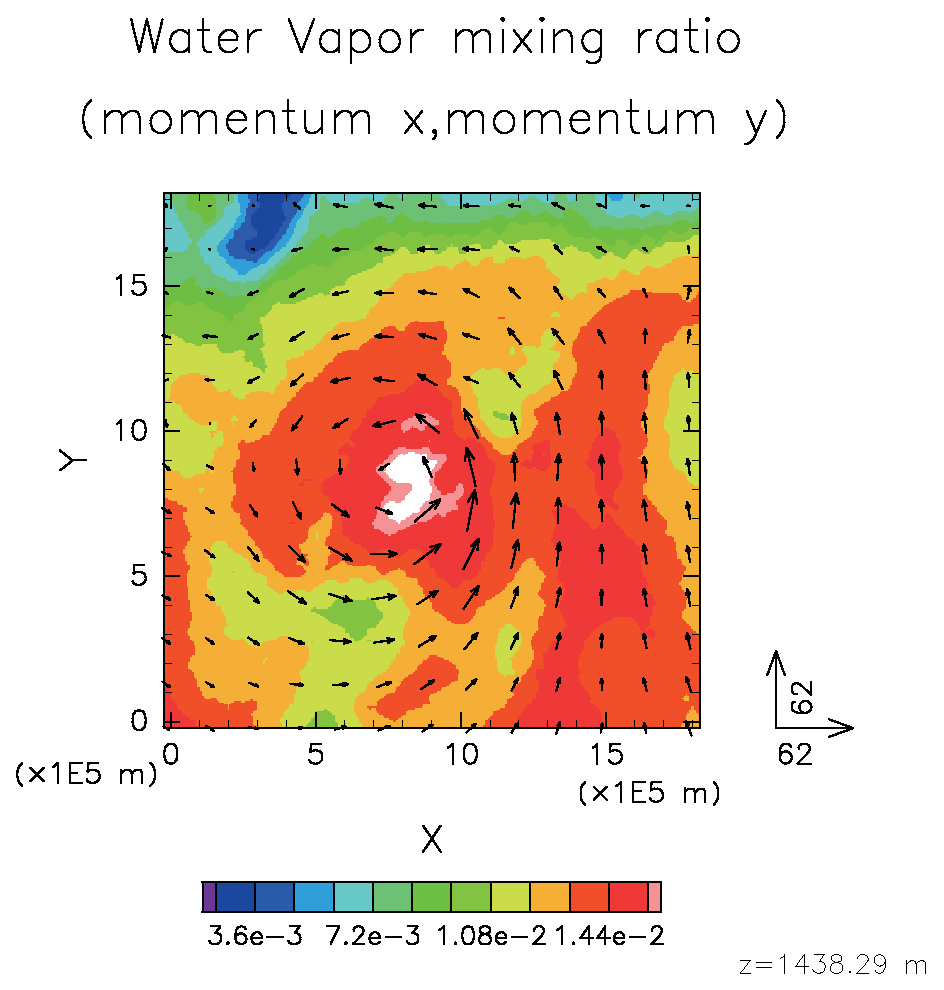
\includegraphics[width=0.7\hsize]{./figure/init_qv-momxy.eps}\\
  \caption{チュートリアル実験の高さ1500mにおける初期場の様子.カラーシェードは比湿,
           ベクトルは水平運動量フラックスを表している.}
  \label{fig:init}
\end{center}
\end{figure}

